\chapter{Desenvolvimento do Aplicativo}\label{chp:des}

\section{Análise de Viabilidade}

Após identificar os elementos e mecânicas de gamificação mais adequados, é crucial avaliar a viabilidade, usabilidade e eficácia dessa abordagem na prática. Isso pode ser feito por meio de projetos piloto, com um número limitado das crianças e por um período definido, para testar a aplicabilidade da proposta gamificada. É importante observar se a abordagem é viável dados os recursos disponíveis e se realmente agrega valor à experiência de aprendizagem matemática dos alunos. A facilidade de uso e entendimento das mecânicas por partes dos alunos também deve ser considerada. E a eficácia pode ser medida por meio de avaliações antes e depois da intervenção, observando se houve maior engajamento e melhores resultados de aprendizagem. Assim, é possível avaliar criticamente os pontos fortes e fracos da abordagem gamificada proposta.

\section{Levantamento de Requisitos}

A gamificação pode ser uma estratégia valiosa para engajar e motivar alunos com síndrome de Down no aprendizado de matemática. Mas para isso, é preciso identificar cuidadosamente quais elementos gamificados se aplicam a este público e seus requisitos específicos. Como muitos têm dificuldade com atividades muito complexas, os desafios e recompensas devem ser graduais e dar ênfase ao processo, não somente aos resultados.

Mecânicas que estimulem a repetição, como níveis que se repetem com aumento progressivo da dificuldade, podem ajudar no aprendizado dos conceitos matemáticos. Elementos visuais, sonoros e táteis devem ser incorporados para aproveitar as habilidades preservadas dos alunos com síndrome de Down. O feedback positivo frequente e as recompensas imediatas também são importantes para manter o engajamento. Identificar o estilo de aprendizagem de cada aluno e escolher mecânicas gamificadas alinhadas a isso é essencial. Assim, a gamificação poderá tornar o aprendizado matemático mais motivador e eficiente para alunos com síndrome de Down.


\subsection{Identificação dos Requisitos}


Os requisitos funcionais (RF) para o aplicativo educacional visam definir as funcionalidades centrais que devem ser implementadas, como autenticação e gerenciamento de usuários, progressão por sessões de jogos, sistema de pontuação e recompensas e gerenciamento de perfil. 
Já os requisitos não funcionais (RNF) estabelecem atributos de qualidade e restrições técnicas, incluindo usabilidade com design intuitivo, compatibilidade multiplataforma, performance otimizada, segurança da informação, manutenibilidade, alta disponibilidade e privacidade dos dados do usuário.

\begin{itemize}
    \item \textbf{Requisitos Funcionais}
    \begin{itemize}
        \item \textbf{RF01:} A aplicação deverá persistir os dados do usuário.

        \item \textbf{RF02:} O usuário poderá entrar na aplicação por meio de autenticação.

        \item \textbf{RF03:} Entrar na na aplicação sem nenhum tipo de autenticação(Os dados não serão persistidos).

        \item \textbf{RF04:} Caso tenha perdido a senha, será enviado um token por email para atualizar a senha

        \item \textbf{RF05:} O aplicativo terá uma opção para atualizar a senha caso o usuário necessite

        \item \textbf{RF06:} O usuário poderá visualizar todo seu histórico de progresso, de todas as suas sessões

        \item \textbf{RF07:} Ao entrar na aplicação, estará visível para o usuário seu progresso atual.

        \item \textbf{RF08}: Exibir tela inicial, com todas as opções disponíveis para o usuário.

        \item \textbf{RF09:} O usuário terá acesso a uma “Loja”, onde poderá comprar avatares com os pontos adquiridos com o jogo.

        \item \textbf{RF10:} Exibir todos os avatares disponíveis para compra.

        \item \textbf{RF11}: Comprar avatar com os créditos adquiridos

        \item \textbf{RF12:} Selecionar um avatar previamente comprado como padrão do aplicativo.

        \item \textbf{RF13:} Escolher a sessão disponível. O progresso é gradual, podendo avançar para a próxima sessão somente após completar a sessão anterior.

        \item \textbf{RF14:} Medir o nível do usuário para colocá-lo em uma sessão condizente com seu nível atual.

        \item \textbf{RF15:} Iniciar um “game” da sessão.

        \item \textbf{RF16:} Encerrar o jogo atual, o progresso será salvo apenas se o jogo for finalizado.

        \item \textbf{RF17:} Uma sessão seria como um capítulo que contém vários jogos, ao completar uma sessão o usuário ganha estrelas.

        \item \textbf{RF18:} Ganhar estrelas de acordo com a sessão finalizada.

        \item \textbf{RF19:} Ao concluir um jogo, o usuário receberá um feedback por questão acertada, podendo ter dicas ou explicação. No caso, de uma sessão, será exibido o desempenho geral da sessão.
        
    \end{itemize}
    \item \textbf{Requisitos Não Funcionais}    
    \begin{itemize}

        \item \textbf{RNF01}:Design Lúdico e Colorido: Utilizar um design lúdico, colorido e amigável para atrair e manter o interesse das crianças.

        \item \textbf{RNF02}: Compatibilidade Multiplataforma: Desenvolver o aplicativo para funcionar em dispositivos móveis (iOS e Android) e computadores, aumentando sua acessibilidade.

        \item \textbf{RNF03:} Performance Responsiva: Assegurar que o aplicativo tenha tempos de resposta rápidos e seja responsivo para proporcionar uma experiência fluida.

        \item \textbf{RNF04:} Segurança: Implementar medidas de segurança rigorosas para proteger as informações pessoais das crianças e garantir uma experiência segura.

        \item \textbf{RNF05:} - Manutenção: O código deve seguir boas práticas para permitir fácil manutenção e atualização.

        \item \textbf{RNF06:} - Disponibilidade: O aplicativo deve ter alta disponibilidade, com tempo de atividade mínimo de 99,9%.

        \textbf{RNF07:}  Privacidade: Os dados dos usuários devem ser usados apenas para os propósitos autorizados e sua privacidade deve ser protegida.
    \end{itemize}    
    \item \textbf{Regras de Negócio}

    As regras de negócio (RN) determinam aspectos fundamentais da lógica e fluxos de operação do sistema. Entre elas, simplified sign-on via Google, salvamento condicional do progresso ao login, lógica de pontuação por acertos e bônus, desbloqueio gradual de conteúdo, utilização de pontos em loja virtual, e direcionamento para conteúdo adequado ao nível do usuário.
    \begin{itemize}
        
        \item \textbf{RN01:} O aplicativo realiza a autenticação usando o sistema de autenticação do Gmail, sem a necessidade de criar ou lembrar senhas separadas. Essa opção simplificada de autenticação visa tornar o processo de login mais conveniente e acessível para as crianças com Síndrome de Down.

        \item \textbf{RN02:} Ao realizar login, todo o progresso deverá ser salvo.

        \item \textbf{RN03:} Caso o usuário tenha optado entrar no aplicativo sem login, seu progresso nao será salvo.

        \item \textbf{RN04:} A cada questão respondida corretamente será totalizado X pontos para a conta.  

        \item \textbf{RN05:} Os pontos poderão ser resgatados ao terminar a sessão atual.

        \item \textbf{RN06:} Ao concluir uma seção sem errar nenhuma questão, serão totalizados X pontos bônus.

        \item \textbf{RN07:} Ao responder uma questão corretamente o usuário será redirecionado para a próxima questão.

        \item \textbf{RN08:} Ao finalizar uma seção, a próxima será desbloqueada para ser jogada.

        \item \textbf{RN09:} A pontuação mínima para avançar de etapa é X.

        \item \textbf{RN10:} Os pontos resgatados pelo usuário poderão ser usados para comprar itens na loja.

        \item \textbf{RN11:} O usuário só poderá selecionar a seção da qual seu nível seja compatível.

        \item \textbf{RN12:} O nível do usuário aumenta conforme avança seções.

        \item \textbf{RN13:} Caso o usuário erre X vezes a mesma questão, o aplicativo mostrará dicas.
        
    
    \end{itemize}

    \item \textbf{Diagramas UML}
    \begin{itemize}
        \item \textbf{Diagrama de Casos de Uso}
        \begin{center}
    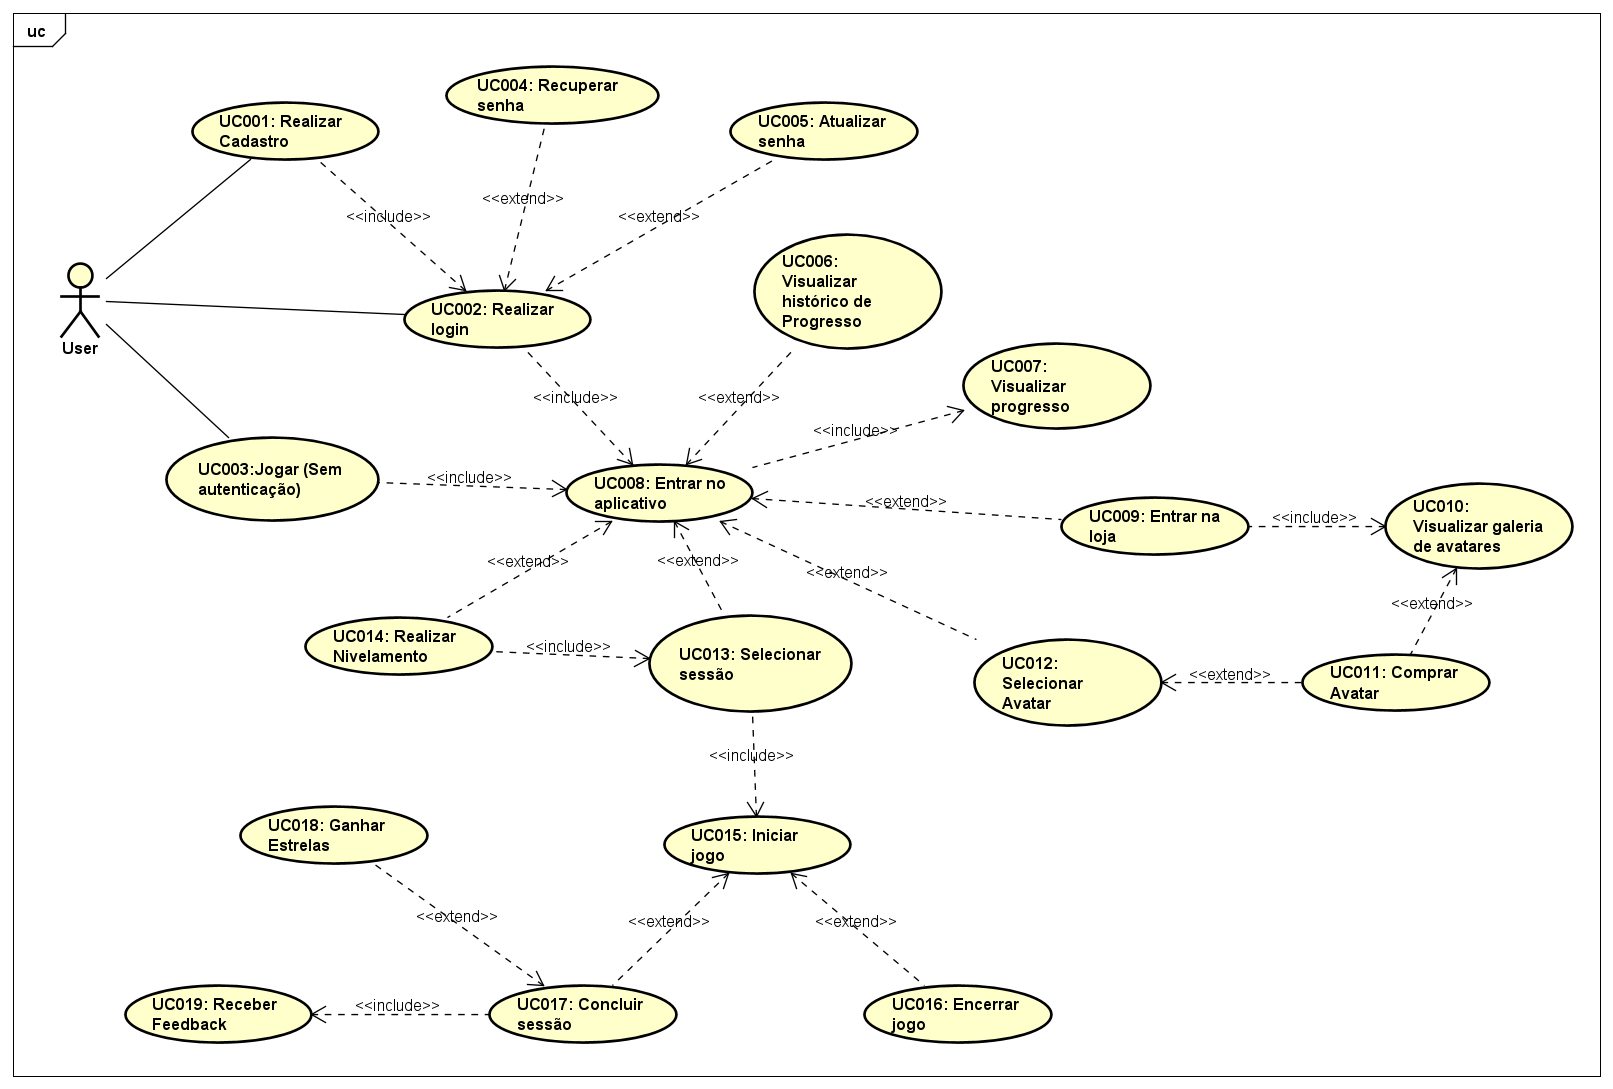
\includegraphics[width=\linewidth]{figuras/UseCase_TCC-1.png}
    \captionof{figure}{Diagrama de caso de uso Fonte: Autores}

    \label{fig:nome-da-imagem}
\end{center}
        \item \textbf{Diagrama de Classes}
        \item \textbf{Diagrama de Atividades}
    \end{itemize}
\end{itemize}

\section{Ferramentas e Tecnologias}

Na presente seção, serão detalhadas as diversas ferramentas e tecnologias empregadas na condução desta pesquisa, desempenhando um papel essencial na coleta, análise e desenvolvimento da pesquisa. A escolha criteriosa desses recursos é fundamental para a robustez e eficácia do estudo, proporcionando uma base sólida para a consecução dos objetivos propostos.

\begin{itemize}

    \item \textbf{React Native} 
    \begin{center}
    
\includegraphics[width=0.5\linewidth]{figuras/React Native.png}
    \captionof{figure}{Logo do framework React Native}
    \label{fig:React Native}
    Fonte para o React Native\footnote{\url{https://reactnative.dev/}}
\end{center}

O React Native é um framework de desenvolvimento de aplicativos móveis que permite a criação de aplicativos nativos para iOS e Android usando JavaScript e React.

A interface foi construída com componentes React Native, possibilitando alta reusabilidade e facilidade de manutenção. O gerenciamento de estado global foi feito via Context API e hooks. Para estilização, usou-se Styled Components com tematização adaptável. A lógica do jogo e regras foram implementadas em JavaScript puro. Atenção especial foi dada à acessibilidade e aspectos cognitivos do público-alvo. O código está organizado seguindo as melhores práticas de React, com componentes pequenos e funções puras. Para qualidade, adotou-se tipagem, testes unitários e integração contínua.No geral, a stack adotada demonstrou alta produtividade e capacidade de entregar uma experiência cross-platform de alto nível e alinhada às necessidades do projeto.

Sobre as versões utilizadas o projeto demonstra o desenvolvimento de um app React Native com recursos avançados de UI, navegação, mídia e animações. O uso do Expo simplifica o setup e configuração do ambiente de desenvolvimento. As versões recentes das principais dependências indicam que o projeto segue as melhores práticas para React Native. No geral, ilustrando um app mobile robusto e bem estruturado utilizando a biblioteca React Native e o ecossistema de ferramentas adjacentes. Utilizando a versão do react 18.2.0 e a versão do react native 0.71.3. 

    \item \textbf{React Native Voice}

    \begin{center}
    
\includegraphics[width=0.5\linewidth]{figuras/React Native Voice.png}
    \captionof{figure}{Logo biblioteca do React Native Voice}
    \label{fig:React Native Voice}
    Fonte para o React Native Voice\footnote{\url{https://github.com/react-native-voice/voice}}
\end{center}

A funcionalidade de reconhecimento de fala foi implementada através da biblioteca open-source react-native-voice, que provê uma API nativa para acesso às funcionalidades de speech-to-text do iOS e Android. A initialização acontece por meio da importação da biblioteca e chamada aos métodos Voice.start() e Voice.stop() para iniciar e interromper o reconhecimento, respectivamente. Configurou-se handlers para os eventos de início e fim da fala, além de tratamento do resultado do texto reconhecido em Voice.onSpeechResults. Após obter a transcrição, ela pode ser utilizada dentro da aplicação React Native, viabilizando diversos usos como entrada de texto por voz e comandos de voz. Optou-se por uma abordagem nativa por ser mais performatica e prover acesso direto às APIs específicas de cada plataforma. A implementação seguiu as melhores práticas recomendadas na documentação da biblioteca, garantindo robustez e experiência transparente entre Android e iOS.
    \item \textbf{Expo}
    \begin{center}
    
\includegraphics[width=0.5\linewidth]{figuras/Expo Framework.jpeg}
    \captionof{figure}{Logo do framework Expo}
    \label{fig:Expo}
    Fonte para o Expo Framework\footnote{\url{https://expo.dev/}}
\end{center}

O Expo é uma plataforma para simplificar o desenvolvimento de aplicativos móveis, especialmente em React Native. Ele oferece facilidade de configuração, desenvolvimento sem necessidade de compilação, bibliotecas prontas para uso e ferramentas como o Expo Client para testar aplicativos de forma rápida. O Expo é uma escolha popular para desenvolvedores que buscam uma abordagem simplificada e eficiente no desenvolvimento móvel.

    \item \textbf{Firebase}
    \begin{center}
    
\includegraphics[width=0.5\linewidth]{figuras/Firebase.png}
    \captionof{figure}{Logo do Firebase}
    \label{fig:Firebase}
    Fonte para o Firebase\footnote{\url{https://firebase.google.com/}}
\end{center}

O Firebase é uma plataforma de desenvolvimento de aplicativos da Google que oferece uma variedade de serviços prontos para uso, como autenticação, banco de dados em tempo real, armazenamento de arquivos, hospedagem e mensagens em nuvem. Ele simplifica o desenvolvimento, permitindo que os desenvolvedores integrem funcionalidades essenciais aos seus aplicativos sem a necessidade de configurar servidores complexos. O Firebase é conhecido por sua facilidade de uso e escalabilidade, sendo uma escolha popular para o desenvolvimento rápido de aplicativos web e móveis.

O Firebase fornece uma excelente plataforma de backend como serviço (BaaS) para o projeto. Ele permite o armazenamento de dados na nuvem em tempo real, autenticação de usuários, notificações push e análise de dados, entre outros recursos. Isso simplifica muito o desenvolvimento do aplicativo, pois lida com toda a infraestrutura do backend. Além disso, tem integração nativa com dispositivos Android e iOS, o que é ideal para este projeto mobile. Como o foco está na experiência de aprendizado gamificada, permite que a equipe se concentre na construção da melhor interface e jogabilidade sem se preocupar com complexidades de backend. Portanto, é uma excelente escolha como BaaS para este projeto educacional.
    \item \textbf{TypeScript}
    \begin{center}
    
\includegraphics[width=0.5\linewidth]{figuras/TypeScript.png}
    \captionof{figure}{Logo do TypeScript}
    \label{fig:TypeScript}
    Fonte para a documentação do TypeScript\footnote{\url{https://www.typescriptlang.org/docs/handbook/typescript-in-5-minutes.html}}
\end{center}

O TypeScript é uma linguagem de programação amplamente adotada no desenvolvimento de aplicativos web e mobile. Sua popularidade se deve ao fato de ser um superconjunto tipado do JavaScript, agregando segurança e produtividade à linguagem original. Quando combinado ao framework React Native, o TypeScript se mostra uma excelente escolha para projetos mobile.

Uma das principais vantagens de utilizá-lo com React Native é a capacidade de reaproveitar código entre plataformas. Como o TypeScript é compilado para JavaScript, linguagem nativa do React Native, os desenvolvedores conseguem compartilhar a maior parte do código entre iOS e Android. Isso aumenta a eficiência no desenvolvimento de apps multiplataforma.

Além disso, Typescript possui um vasto ecossistema de bibliotecas e frameworks, incluindo aqueles voltados para React Native. Essas ferramentas facilitam a implementação de recursos como animações, gerenciamento de estado e integração com APIs. A comunidade ativa contribui com tutoriais, documentações e fóruns de discussão, provendo amplo suporte ao desenvolvimento.

Ao optar pelo Typescript com React Native, os desenvolvedores garantem uma linguagem versátil e uma plataforma robusta para a criação de apps modernos e de alta qualidade. A união dessas tecnologias permite um fluxo ágil e produtivo, entregando ao usuário final uma experiência enriquecida. Portanto, o Typescript se consolida como uma ótima escolha para projetos mobile com React Native.

O projeto é um exemplo de aplicação das modernas práticas de desenvolvimento de software. Ele segue uma arquitetura modular, que permite uma maior facilidade de manutenção e extensão do código. O projeto é todo escrito em TypeScript, uma linguagem que oferece segurança de tipo e evita erros comuns em JavaScript.
Além disso conta com o apoio de diversas bibliotecas de terceiros, que fornecem funcionalidades adicionais, como gerenciamento de estado com Redux, roteamento com React Navigation, persistência de dados com AsyncStorage, entre outras. Para garantir a qualidade e a confiabilidade do código, o projeto possui uma suíte abrangente de testes, que utiliza ferramentas como Jest, Enzyme e Detox, facilitando o desenvolvimento e manutenção da aplicação em si.

Por que TypeScript?

    O TypeScript é uma variação do JavaScript que traz benefícios como:

    Tipagem Estática: Ajuda a evitar erros comuns, tornando o código mais claro.

    Melhoria na Segurança e Eficiência: O compilador pode detectar e corrigir erros de tipo em tempo de compilação, economizando tempo na depuração.

    Escalabilidade: Torna o código mais modular e reutilizável, melhorando a escalabilidade.

    \item \textbf{Astah UML}
    \begin{center}
    
\includegraphics[width=0.5\linewidth]{figuras/Astah UML.png}
    \captionof{figure}{logo da ferramenta para criação de UMLs AstahUML }
    \label{fig:Astah UML}
    Fonte para o AstahUML\footnote{\url{https://astah.net/products/astah-uml/}}
\end{center}

O Astah UML é uma ferramenta de modelagem UML (Unified Modeling Language) que oferece recursos abrangentes para profissionais de software, analistas de sistemas e outros envolvidos no desenvolvimento de software. Ele suporta todos os principais diagramas da UML, incluindo diagramas de classe, sequência, atividade, estado, e muito mais. Isso permite que os usuários visualizem e documentem diferentes aspectos de um sistema.
    \item \textbf{Figma}
    \begin{center}
    
\includegraphics[width=0.5\linewidth]{figuras/Figma.png}
    \captionof{figure}{logo da ferramenta de Design Figma}
    \label{fig:Figma}
    Fonte para o Figma Fonte\footnote{\url{https://www.figma.com/}}
\end{center}

O Figma é uma plataforma de design colaborativo baseada na web que revoluciona a maneira como equipes de design trabalham. Permitindo colaboração em tempo real, prototipagem interativa e a criação de bibliotecas de componentes reutilizáveis, o Figma oferece uma abordagem flexível e centrada na equipe para o design de interfaces de usuário (UI) e experiência do usuário (UX). Sua facilidade de uso, ampla compatibilidade com formatos de arquivo e integração fluida com outras ferramentas fazem dele uma escolha popular para profissionais de design e desenvolvimento em todo o mundo.

O Figma foi utilizado para diagramar os wireframes das principais telas e fluxos de navegação do aplicativo. Isso permitiu testar rapidamente como o usuário interage com os elementos de gamificação e conteúdos didáticos já neste estágio inicial. O wireflow desenvolvido no Figma serviu como guia para o desenvolvimento visual e codificação do aplicativo, garantindo que o produto final atendesse às necessidades dos usuários. O protótipo interativo criado também facilitou testes com usuários reais ainda nas fases iniciais do projeto e serviu como base para a evolução da aplicação, fornecendo feedback valioso antes de escrever qualquer linha de código a fim de validações. Seguimos o layout fornecido como base para a implementação. 

Os fluxos de navegação também ajudam a comunicar a jornada do usuário para a equipe, pois permitem visualizar o caminho que um usuário irá percorrer ao realizar determinadas ações. A combinação de wireframes e fluxos de navegação no Figma torna a prototipação uma etapa crucial no processo de design, permitindo uma melhor compreensão das interações e proporcionando uma base sólida para o desenvolvimento do produto.
   
\end{itemize}

\section{Prototipação de telas}

A prototipação de telas é uma etapa importante no design de aplicativos e sites, que permite simular a experiência do usuário antes mesmo de construir o produto final. O protótipo consiste em um modelo interativo das telas, contendo os fluxos de navegação e os elementos de interface. Ele pode ter diferentes níveis de fidelidade, desde esboçosSimples até designs mais refinados. 

A grande vantagem da prototipação é permitir testar e validar ideias de forma rápida e barata, identificando problemas na experiência do usuário precocemente, antes de partir para a programação. Ferramentas como Figma, Adobe XD e Proto.io facilitam a criação de protótipos clicáveis que simulam os comportamentos da interface. Com testes iterativos envolvendo usuários reais, o protótipo é aprimorado até chegar em um design pronto para ser desenvolvido. Dessa forma, a prototipação ajuda a economizar tempo e evitar retrabalho no processo de design.

\subsection{Desenvolvimento do protótipo}


\begin{itemize}
    \item \textbf{Participantes e procedimentos da avaliação do protótipo}
    \item \textbf{Validação: testes de usabilidade, observação de uso, feedback dos usuários}
    
\end{itemize}

\section{Repositório}

O que é um Repositório?

Um repositório no GitHub é como um cofre para seu projeto. Ele contém todos os arquivos do seu projeto, além do histórico de todas as alterações feitas ao longo do tempo. É como uma versão online do seu projeto que facilita a colaboração e o controle de versões.

Estrutura do Repositório

Branches

No contexto do GitHub, usamos "branches" para criar diferentes versões do projeto. Cada branch é uma ramificação independente do código-fonte, possibilitando que você isole e desenvolva novas funcionalidades, refatore o código ou faça correções e testes em paralelo, sem interferir no código existente na branch principal, que geralmente é nomeada como \textit{main} \cite{al}. Neste projeto, utilizamos apenas a branche \textit{main}.


Refatoração e Aprimoramento

Uma análise crítica da estrutura existente levou a mudanças significativas. A reestruturação do código, adotando melhores práticas e aprimorando a arquitetura. Bem como a criação de uma nova branche nomeada de develop ...................

E o projeto ficou organizado da seguinte maneira: 

Branche main

............

Branche develop

..............

Versionamento do Código

Versão 0.0.1 -  Criação do projeto.

Versão 0.1.0 - Organizamos as pastas de forma mais lógica. Cada tipo de funcionalidade agora tem seu próprio espaço. Para facilitar a compreensão e manutenção do código.

Versão 0.2.0 - Componentização. Dividimos os componentes em partes menores, cada uma realizando uma tarefa específica. Isso ajuda na organização e na compreensão do código.

Versão 0.3.0 - Separamos os arquivos de estilo, proporcionando uma consistência visual melhor.

Versão 0.4.0 - Movemos o gerenciamento de estado para "stores", proporcionando uma prática recomendada para projetos React Native.

Versão 1.0.0-alpha - Decidimos mudar a tecnologia utilizada de JavaScript para TypeScript.


Onde usar??  ->  Essas mudanças visavam criar uma base de código mais organizada, fácil de entender e pronta para receber atualizações e melhorias no futuro. Este projeto, agora utilizando TypeScript e seguindo melhores práticas, está mais preparado para crescer de maneira sustentável e com qualidade.


        
